\section{Sub controllers}
This section will aim to derive sub controllers for the boat lift safety control system. The sub controllers communicate with each other and externally through the interactions and signals desribed in the previous section:

\begin{enumerate}
	\item Master controller, controls the water flow and water level of the lift
	\item Gate controller, controls the lift gates
	\item Valve controller, controls the lift valves
	\item Signal controller, controls the signal lights
\end{enumerate}

\noindent The functioning of the sub controllers in combination with the actions and signals is displayed in the figure below:

\begin{figure}[!h]
	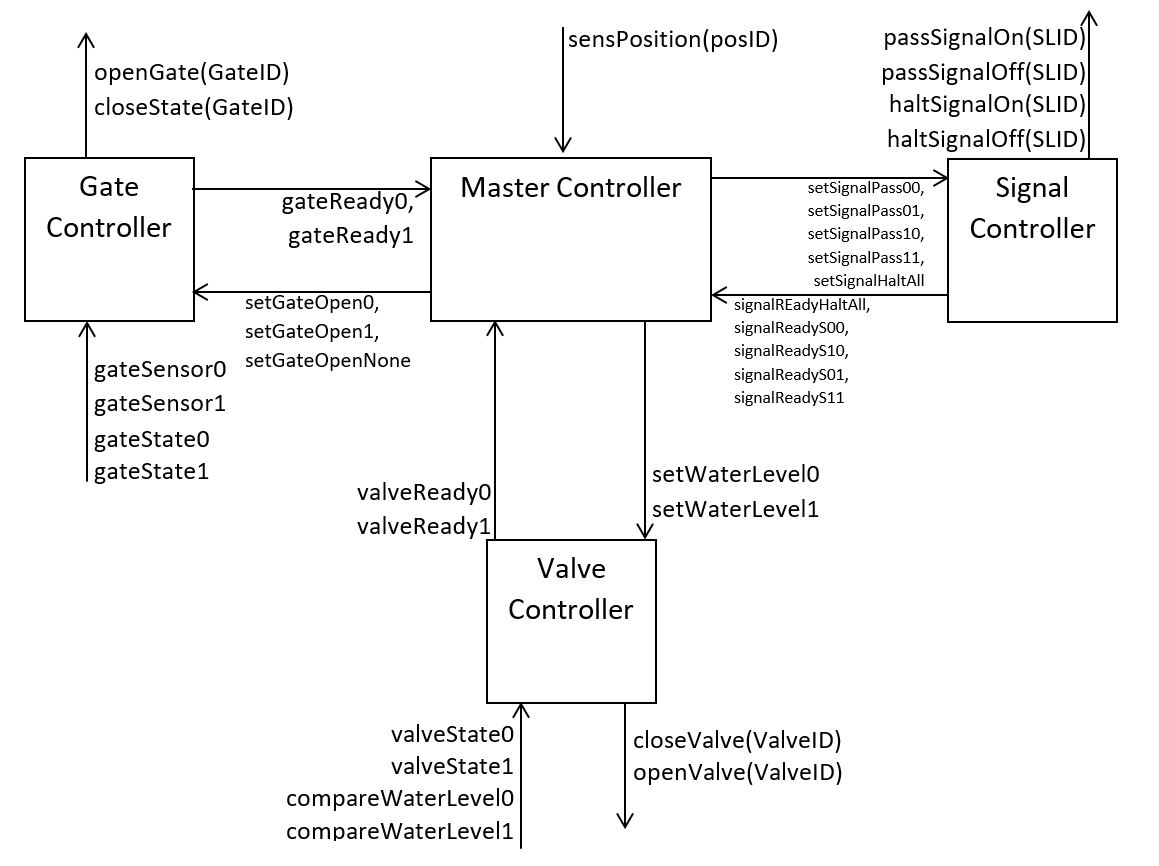
\includegraphics[width=\linewidth]{controllers}
	\caption{Scheme of sub controllers}
	\label{fig:subcontrollers}
\end{figure}
\subsection{Master controller}
Master controller keeps track of the position of the ship inside the system. Its responsible for coordinating the sequence of actions that are executed. These are either to set the gates, valves or signals. It gets confirmations or error signals back from the other sub controllers to either confirm or refute actions were carried out. \\

\noindent In Table \ref{tab:internal} a list of internal commands which the master controller uses to communicate with other sub controllers is displayed.

\begin{table}[htbp]
	\centering
	\begin{tabular}{lll}
		\toprule
		\textbf{Internal actions} & \textbf{Description} & \textbf{Parameter} \\
		\midrule
		setSignalPass & Set given signal to pass & \{0, signalID\} \\
		setWaterLevel & Set the waterlevel to given level & Level\\
		setGateOpen & Open the given gate & \{0, gateID\} \\
		signalReady & setSignalPass successful & None\\
		signalError & setSignalPass not successful & None \\
		gateReady & setGateOpen successful & None\\
		gateError & setGateOpen not successful & None\\
		waterLevelReady & setWaterLevel successful & None\\
		waterLevelError & setWaterLevel not successful & None\\
		\bottomrule
	\end{tabular}%
	\caption{Internal commands}
	\label{tab:internal}%
\end{table}%

\subsection{Gate controller}
The gate controller ensures the safety requirements are met. It gets a close or open command for the gates from the master controller. It sends a Gateready signal back to the master to confirm a gate has been safely opened or closed. 
\subsection{Valve controller}
The valve controller gets setWaterlevel command from the master controller to set the waterlevel to be equal to container x.1. It receives the waterflowstate\_ID and valvestate\_ID to know if a valve is either open or closed or there is is water flowing through the valve. It executes the external actions openValve\_ID and closeValve\_ID to actually open or close a valve.  
\subsection{Signal controller}
The signal controller receives a SetSignalPass\_ID from the master controller. It sends back that the signal has been set with Signalready or Signalerror when this was not accomplished. The signal subcontroller executes the external action SetSignalHold\_ID or SetSignalPass\_ID to set the signal lights. 
